\chapter{Re-curation and rational enrichment of knowledge graphs in Biological Expression Language}
\label{ch:recuration}

\section*{Preface}

Following Chapters~\ref{ch:pybel} and~\ref{ch:belcommons}, which laid the groundwork for handling and exploring knowledge graphs encoded in \ac{BEL}, the following publication describes the development and application of two workflows for 1) ensuring the quality of knowledge graphs encoded in \ac{BEL} and 2) enriching these knowledge graphs with semi-automated curation that leverages large-scale information extraction and natural language processing systems.
It presents an evaluation and comparison to previous semi-automated curation workflows using the metrics for curation overhead and efficiency described by Rodr\'{i}guez-Esteban~\cite{Rodriguez-Esteban2015}.

\vspace*{\fill}

Reprinted with permission from "Hoyt, C. T. \textit{et al.}. (2019) Re-curation and rational enrichment of knowledge graphs in Biological Expression Language. \textit{Database}, 2019, baz068".
Copyright © Hoyt, C. T., \textit{et al.}, 2019.

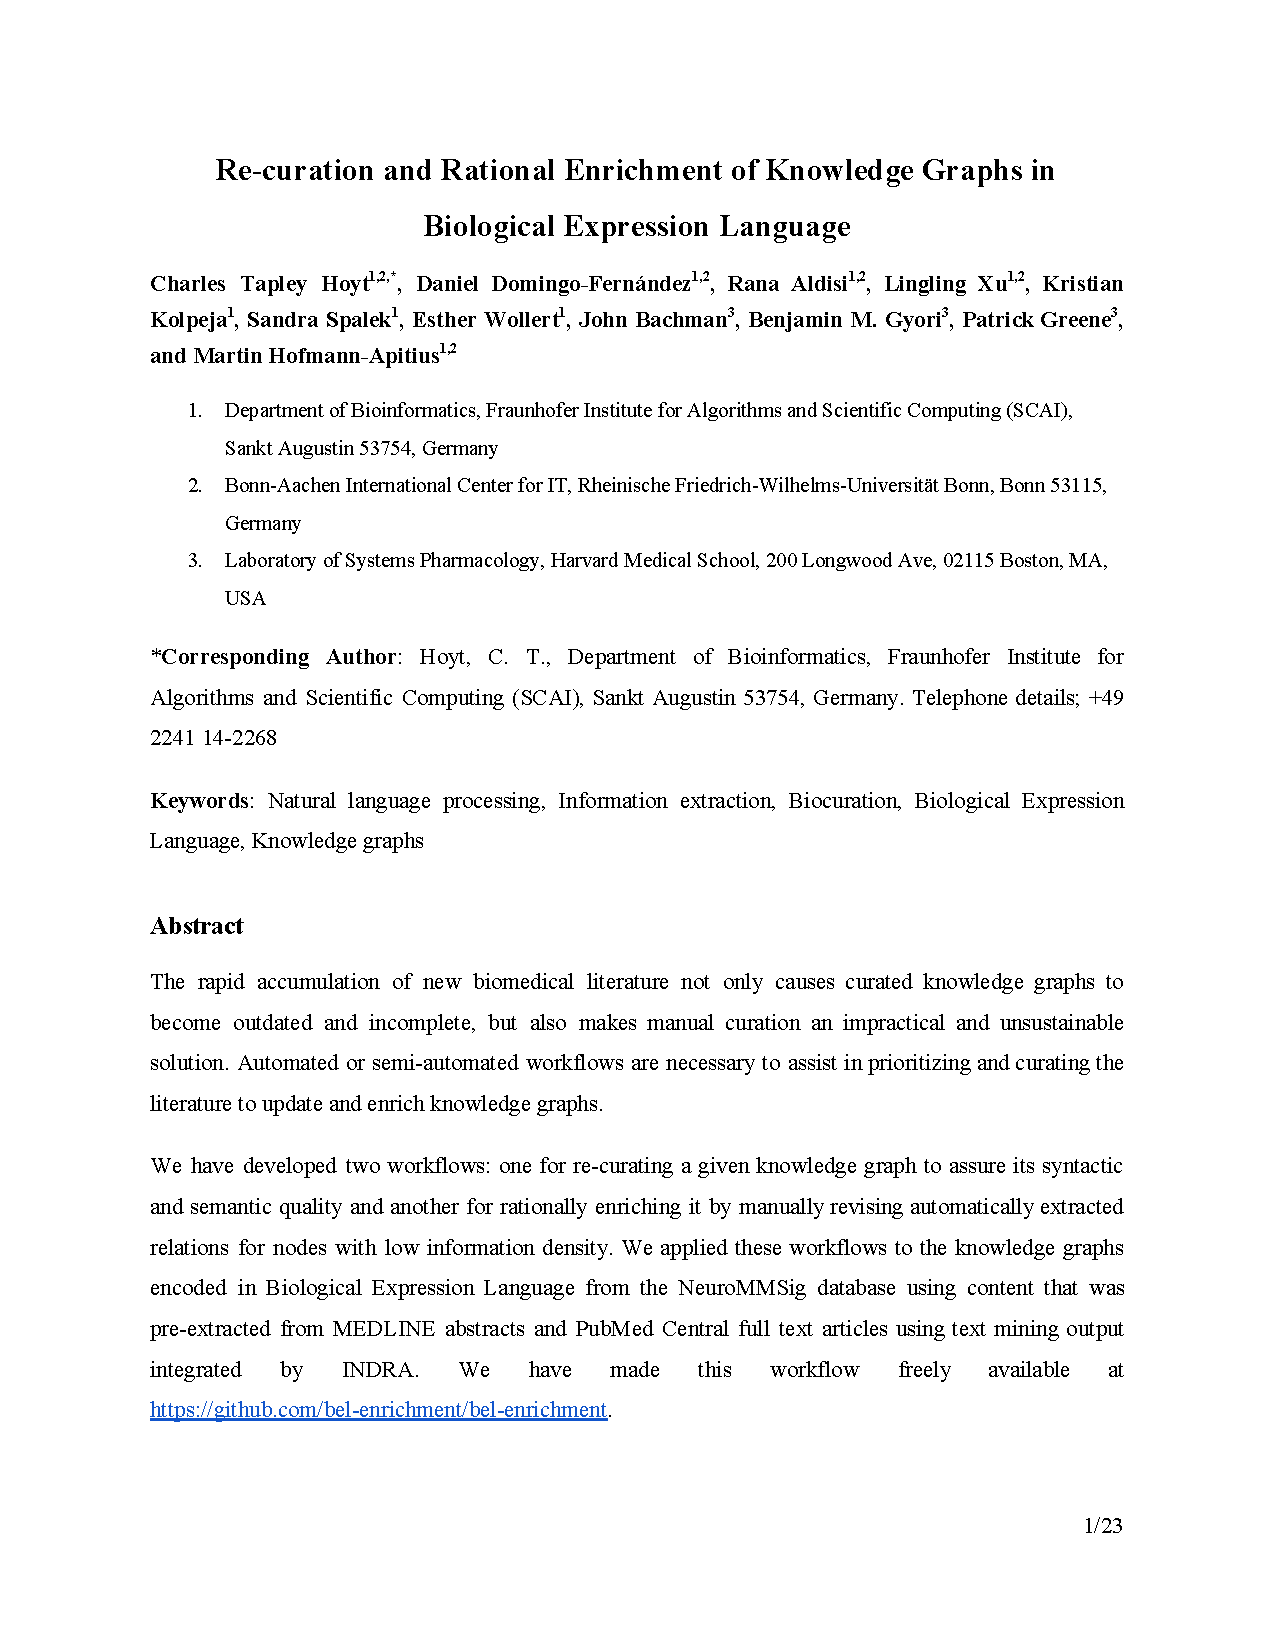
\includepdf[pages={-}]{articles/recuration.pdf}

\section*{Postface}

Continuing with the goals of developing the ecosystem around \ac{BEL} and PyBEL, the workflows and all resulting manually curated results from this publication have been made freely and openly available to the community.
The first workflow for quality control of \ac{BEL} promotes more sustainable curation practices through the usage of version control systems and continuous integration systems.
It was used to re-curate all of the knowledge assemblies from the AETIONOMY project as well as enforce the clean generation of new knowledge during the Human Brain Pharmacome project that can be found at \url{https://github.com/pharmacome/knowledge}.
Without re-curation, previously generated content may neither be syntactically, semantically, nor biologically correct.

The second workflow allows for the usage of massively extracted content from unstructured text and automated enrichment of knowledge graphs, which further reduces this burden.
Ultimately, the usage of these workflows provided significant improvements over both manual curation and previously published state-of-the-art semi-automated curation systems.
These improvements manifested across all of the management, planning, and reading aspects of curation.
The workflow is scalable because pre-extraction can be done once in bulk, then on a schedule so the most recent content is always available.
Further, because curation of each statement is independent, the workflow is scalable with respect to number of curators.
Then, between each curation, the priorities of all statements can be updated.

While enrichment can be applied generally to any disease- or pathways-specific knowledge graph, it can also be iterated with topic-driven or publication-driven curation to quickly acquire breadth in new fields.

Finally, the conclusion of this publication noted that a spreadsheet-based curation workflow has the benefit of being simple.
Its conceptualization has motivated some improvements to the INDRA Database\footnote{\url{https://db.indra.bio}} web application that will likely result in its evolution into a web-based curation application.
When interfacing directly with the database, the workflow described in this article can be implemented directly.
Other community driven curation tools like WikiPathways and the SBV Improver may be able to draw content from this system or make contributions directly to improve their efficiency.
